\documentclass[a4paper,12pt]{scrreprt}

\usepackage[english]{babel}
\usepackage[utf8x]{inputenc}
\usepackage{ucs}

\usepackage{hyperref}

\usepackage{graphicx}
\usepackage{float}

\title{Kingdom of Kush - 0 A.D. Mod - Specification}

\begin{document}

\maketitle

\abstract{This is the development specification for the Kushite Mod. The Kushite Mod adds the Kushite civilization to the real time strategy game \href{https://play0ad.com/}{0 A.D.}.}

\tableofcontents

\chapter{Units, Buildings and Technology Tree}

Buildings:

\begin{itemize}
	\item Temple
	\item Civic Center
	\item Storage Depot $\rightarrow$ TODO Research \& Sketch
	\item House
	\item Blacksmith $\rightarrow$ TODO Sketch
	\item Fields
	\item Farm
	\item Stable
	%\item (TODO Something like a Mill)
	\item Marketplace $\rightarrow$ TODO Sketch
	\item Trader (land)
	\item Fisher Boat $\rightarrow$ TODO Research (papyrus or wooden?) \& Sketch
	\item Light Warship
	\item Medium Warship
	\item Dock
	\item Diplomacy Center $\rightarrow$ TODO Research (where/how did they hire mercenaries?)
	\item Garrison/Barrack $\rightarrow$ TODO Research (how did they look like?)
	\item Fortress
	\item Tower
	\item Wall
	\item Wonder
\end{itemize}

Units:

\begin{itemize}
	\item Woman worker $\rightarrow$ TODO Research (how did they look like? Avoid racial bias)
	\item Basic infantry/cavalry workers $\rightarrow$ TODO Research (how did they look like?)
	\item Chariots
	\item Beja Swordsman (mercenaries)
	\item Beja Camel Warrior (mercenaries)
	\item Siege Weapons
	\begin{itemize}
		\item Battering Ram
		\item Siege Tower
	\end{itemize}
	\item Elite Units
	\begin{itemize}
		\item Nubian Bowmen
		\item TODO other elite units
	\end{itemize}
	\item Heros $\rightarrow$ TODO Research (Important Queens/Kings, Priests etc.)
\end{itemize}

Special Technologies:

\begin{itemize}
	\item Iron production bonus
	\item Cattle bonus
\end{itemize}

Agriculture:

\begin{itemize}
	\item Wheat fields
	\item Animals
	\begin{itemize}
		\item Sanga Cattle
		\item Goat
	\end{itemize}
\end{itemize}
Special Features:

\begin{itemize}
	\item Nubian Bowmen shoot poisoned arrows
\end{itemize}

\section{Buildings}

\subsection{Temple}

\subsection{Civic Center}

\subsection{Storage Depot}

\subsection{House}

\section{Units}

\subsection{Chariot}

\section{Common Misconception}

\subsection{War Elephants}

Short answer: no, they did not use them.

TODO Long answer

\section{Weaknesses and Strengths}

All this reading has made a few things clear to me. The Kushites had particular strengths and weaknesses relevant to the game-play of 0AD.

Weakness:

\begin{itemize}
	\item Weak armor: Basic units barely used armor. Special units, champions and heroes have (quality) quilted cotton and scale armor, but they should be relatively expensive.
	\item Weak navy. Apparently no real seafaring capability (which means they’d be a weak choice for an island map). But they did have boats, and transport of troops, and basic naval defense is a definite yes. Weak boats can be compensated with garrisons of archers, firing volleys of flaming arrows (fig. 7a).
	\item Weak siege equipment: Only cursory mention of siege equipment and tactics, which include ladders, ship-masts, sapping attacks on walls, but also siege towers and battering rams.
\end{itemize}

Strength:

\begin{itemize}
	\item Infantry should have a speed bonus, because low armor makes them faster (and cheaper)

	\item Their cavalry should be particularly strong and fast. Highly desired by the Egyptians and Assyrians, the specific breed of Kushite horses was large, fast and strong. I believe it is the ancestor to the rare Dongola, or Dongolawi horse, an important breed throughout the greater Sudan in later times (disregard Wikipedia on this one. Their page dismisses the Sudanic origin of this breed, apparently based on the axiom that horses were introduced to Sudan in much later times. By now we know they were being bred by the 2nd millennium BCE, but this isn’t common knowledge I guess. In addition, the page fails to distinguish, or even identify the unique physical features of this breed. The author seems to be conflating barb and Arab horses with older African breeds).

	\item Fast chariots (drawn by two horses), shooting accurate volleys of arrows. Perfect for hit and run tactics.

	\item Large-scale food production, due to irrigation and cattle herding. Allows recruiting many, fast and cheap units early in the game, ideal for early raiding.

	\item Strong buildings and defenses. Thick walls of cut stone, dry-stone or fired brick. Mud-brick foundations provide a certain plasticity, which in turn ensures the stability of larger structures.

	\item Strong weapons. Early iron (steel) production gives them strong swords, spears and arrow tips. Maybe they should have a weak defense, but a strong attack.

	\item They were world renowned for their archery skills for several millennia. They should be the most accurate archers in the game. Even in later times, Heliodorus of Emesa mentions their “unerring skill in hitting their target, their adversaries’ eyes”. This was repeated by the invading Arabs of the Rashidun Caliphate, who called them “pupil smiters”, and were forced to retreat from Sudan with many eyes lost (battle of Dongola).  
\end{itemize}

\chapter{Art and Design}

\section{Color Palette}

\section{Textures}

\chapter{Miscellaneous}

\section{Licenses}

\begin{itemize}
	\item Code: GPL v2
	\item Documentation: GPL v2 (excluding images)
	\item Images: Creative Commons
	\item 3D-Models?
	\item Sound?
\end{itemize}

\chapter{The Kingdom of Kush: A proper introduction}

\begin{center}
\textit{“Oh Great God, swift one. Who comes to him who calls. Watch my sister for me, the woman born in the same womb as me. Do for her as I have done for you. Spontaneous miracles that cannot be denied. Elevate her children and make them prosper, even as you did for me.”}\\[12pt]

\noindent
-From Taharqa’s prayer to Amun, at his temple in Kawa-
\end{center}

\begin{figure}[H]
	\centering
	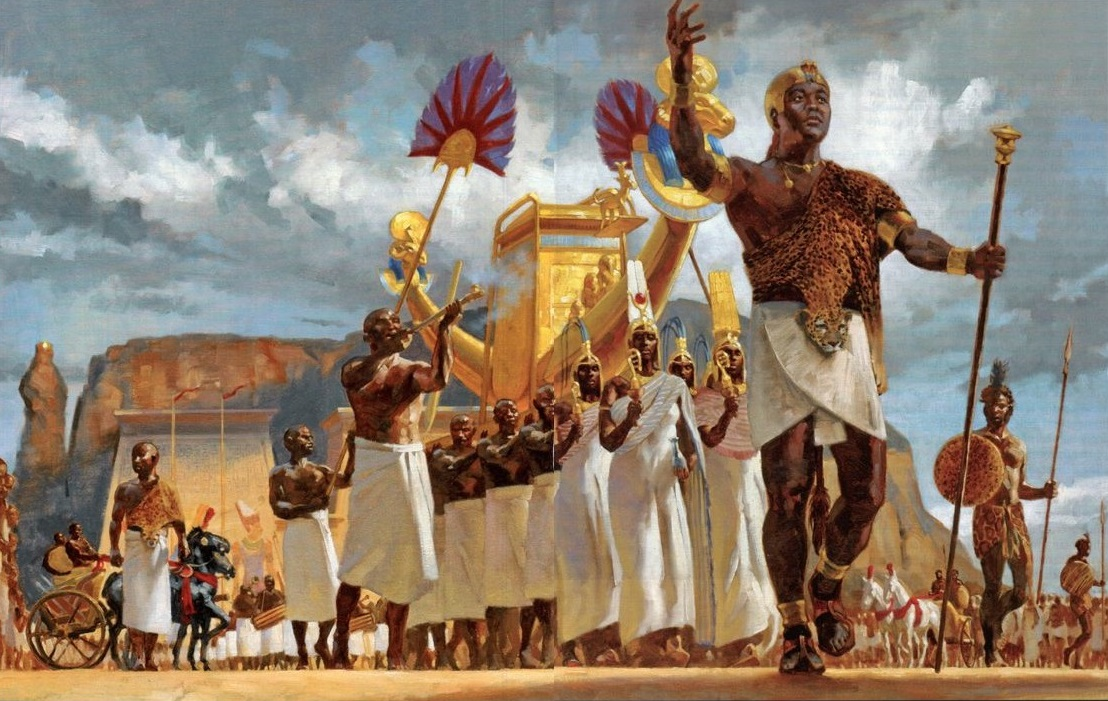
\includegraphics[width=0.8\textwidth]{img/taharqa_pharaoh}
	\caption{Taharqa, pharaoh of the 25th dynasty and father of the later Meroe period, at the temple of Amun in Napata. The holy mountain Jebel (Gebel) Barkal is in the background.}
\end{figure}

Often misunderstood, and even more often overlooked, Kush was a major center of power in the ancient world. Its deserts and its armies were the southern frontier for many classical civilizations. Its gold and ivory were prized throughout the Mediterranean and the Middle East. Its trade routes connected Africa to the rest of the world and its mercenaries served as far as Greece. It’s rulers, many of them powerful queens, known as Kandakes, ruled in the style of the Pharaohs of the New Kingdom. City builders, administrators, craftsmen and artists, ironworkers, priests, warriors, farmers, cattle herders and horse breeders. Builders of pyramids. The bowmen of Nubia. Who where these Kushites, and why would they be such an invaluable addition to 0 A.D.?

\begin{figure}[H]
	\centering
	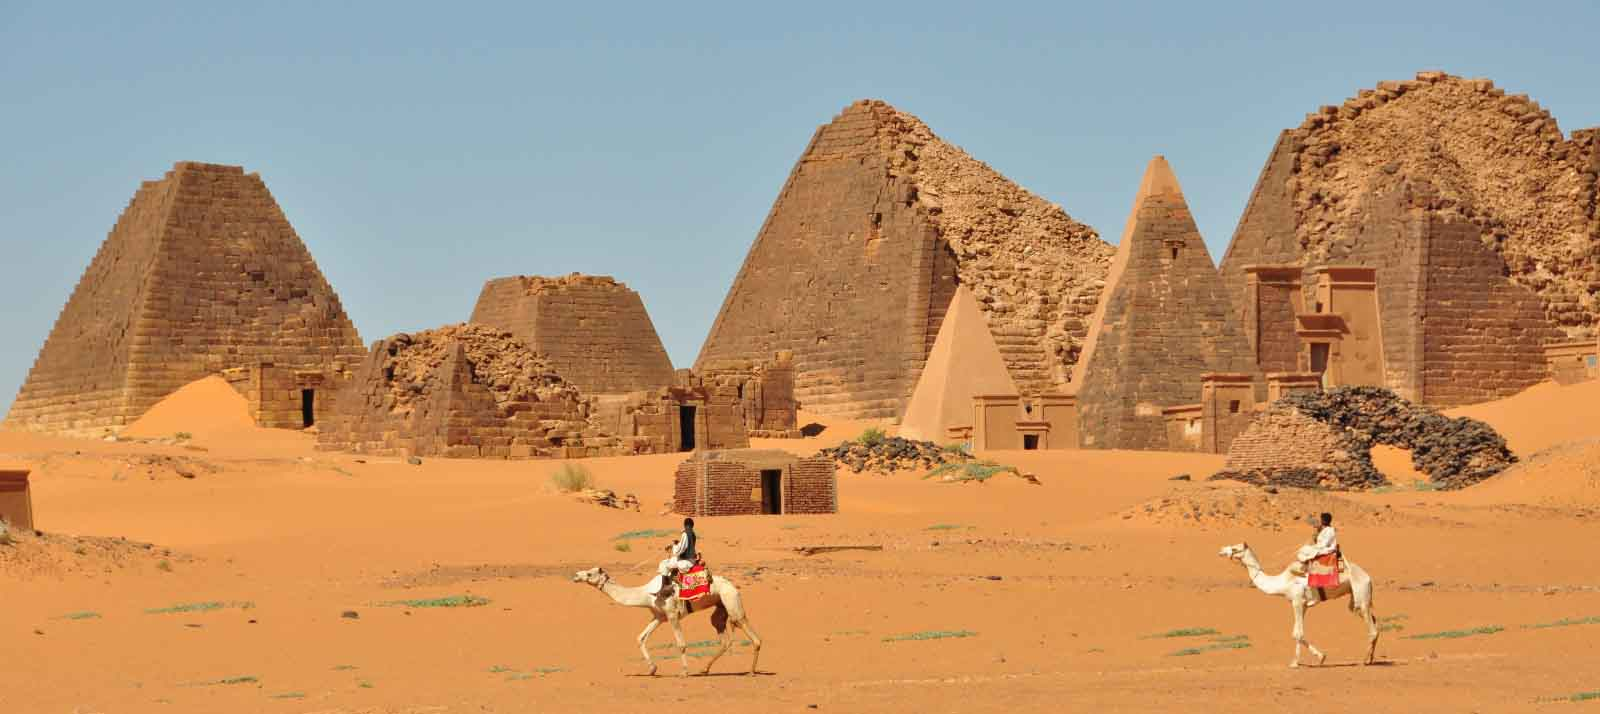
\includegraphics[width=0.8\textwidth]{img/meroe_pyramids}
	\caption{Some of the Iconic Nubian pyramids, at Meroe. Between the 8th Cenury BCE and 350 A.D., 255 pyramids were built by the Kushites, at El Kurru, Napata, Meroe and Nuri}
\end{figure}

Because the Kushites have not yet been properly introduced, I will attempt to provide you with a thorough, yet concise, illustrated analysis of Kushitic history, outlining their origin and environment, culture and religion, architecture, economy and military. As well as contextualizing them in a broader Mediterranean and Middle Eastern world, around the time frame of 0 A.D., including the prolonged wars they waged against several civilizations already featured in the game. Because of the lack of credible and historically accurate representations of these people in popular culture, I have spent some time, gathering a rich collection of historically accurate and relevant images, focused on important archaeological sites, and accurate reconstructions of houses, monuments, cities and the people and attire of various classes and backgrounds within Kush. If any attempt is made to represent “The Kingdom of Kush” in 0 A.D., the images provided in this introduction can provide the backbone for models of buildings and units, as they represent some of the most historically accurate images available on this civilization.

\end{document}